%!TEX root = project.tex

\chapter*{About this project}
\paragraph{Abstract}
The name of the web application I have created is "Heap-Overflow", as the name suggests, it is a web application similar to stack overflow. It is a forum web application that is created using a MERN stack (Mongo, Express, React, Node.js). It has all the features of a CRUD application (Create, Read, Update, Delete), alongside others that will be written about in detail further on in this document. The main intention with creating a forum website with the MERN stack was to familiarise myself more with the main technologies used in the creation of modern day web applications. The MERN stack is one of the most popular frameworks used in the industry and the stack is made up of technologies that allow for the development of very fast, responsive and intuitive web applications, through the use of a variety of libraries, databases and frameworks. These technologies allow the developer to streamline the development of modern day web applications in an intuitive manner. The development of this website also exposed me to technologies such as Postman, which was a very helpful tool in determining whether the back-end of the application was functioning in the manner it was supposed to. This document will go into great detail into the research and the development of the web application "Heap-Overflow".

\paragraph{Authors}
Arnas Steponavicius


\chapter{Introduction}
The objective of this project is to create a forum website which will be called "Heap-Overflow". It will be a web-based application inspired by the likes of popular websites such as "stackoverflow". A decision was made to create a forum web application similar in function to "stackoverflow" in order to improve upon my own skill set and gain more experience and insight in terms of creating web-based applications. I had mulled over a few ideas for this project. The initial concept for this project was creating a web application that would allow users to securely transfer files from one user to another by means of encrypting and decrypting files using a key that could be passed around. However, I ultimately settled on the idea to create a forum website, I will explain my change of plan in the conclusions section of this paper.

Even though I ended up changing project ideas, My objective was still the same as before, I still had a curiosity as to how modern day web applications that have high scalabitility, are created and developed using an assortment of different libraries, frameworks and technologies. With scalable web applications there is always room for improvement, as there are constant iterations and improvements being made to the technologies that create these applications, to deliver users the best possible experience when browsing. As a benefit, this would allow for continuous work on the application in the long term, whether it would be adding extra features to the forum, or refactoring the code to be more efficient and less cluttered in the event a technology that was used got a major update. Forum websites are also an important part of the internet, they allow similar minded individuals to converge into one place and share their ideas, questions and answers amongst each other. As mentioned earlier, forum websites also have the ability to grow further from the initial stages of just creating an account and posting questions, answers or ideas on interesting topics, such as the implementation of different features like learning/teaching sections or a most commonly asked questions section, however at its core, a forum website still mainly focuses on the interaction between the community through asking questions, posting answers and sharing ideas. This was another reason that contributed to creating a forum web application.

While I did choose a technology stack I had previously used, MERN stack, it had been two years since I had last used it and I found myself relearning a lot of the features, since the technologies in the stack got many major updates over that time span. These major updates to the technological stack also came with the addition of new features, which I had to learn about regarding the situations of when to use it. These new features will be expanded on during the technology review section further into this document.
Doing this project with a technological stack that I had previously used also allowed me to improve my skill set with the technologies further. With the M.E.R.N stack being a very popular choice for web application development, this gave me access to a plethora of resources to aid in my journey of developing this project. The MERN stack is a variation of a MEAN stack. The differences in these stack technologies will be discussed in the upcoming technology review section of this paper. As a brief introduction, however I will explain the MERN stack in simple detail, but will also go into further detail during the technology review section. As mentioned in the abstract, the MERN stack consists of four technologies, MongoDB which is a database used to store collections (user details, user posts etc...) from the application, Express and Node.js go hand in hand and are responsible for the server-side operations like routing (letting users change web pages) and finally React.js which is a JavaScript framework that allows the building of complex User Interfaces (UIs) through rendered components (web pages). The system design section will also provide detailed explanations as to how the MERN stack technologies work in tandem in this web application.

The success or failure of this project would be measured, through the responsiveness, design and available features of the web application. Responsiveness represents aspects such as initial loading times for the application, how efficient the application at changing the state of what is shown when links are clicked or when forms are submitted. Design corresponds to the UI that is displayed, criteria for measuring something like UI would include questions such as, "Do the colours clash?" or "Is it too cluttered where the user would have a hard time navigating the page?". A more detailed explanation as to how I tested these things will be talked about in the system evaluation section.
 The link to the repository which explains how to install this project and run it locally on your machine can accessed via this url: https://github.com/ArnasSteponavicius00/heap-overflow. As mentioned at the end of some paragraphs there will also be different sections to this paper which will go into detail about the creation of this project, below are the sections this paper covers.
 \begin{itemize}
     \item Methodology - This section highlights the methods and looks into a variety of approaches and the chosen approach to the development of the project. It also highlights some of the testing, and development tools used during development.
     \item Technology Review - Delves into the different technologies used, researched and considered for the development of the project. It will cover the reasoning behind chosen technologies, their advantages / disadvantages and comparisons between the used technologies and the considered technologies.
     \item System Design - This section is the core part of the paper, it gives insight and explains the code in behind the web application in detail. It will look into how the different elements of the MERN stack interact with each other, how the application is hosted, how the data for the users is stored and authentication.
     \item System Evaluation - Showcases the testing done during the development life-cycle. It will also aim to answer different question such as, "have the goals layed out were achieved?", "where can further improvements be made and are there limitations?". This section will also take a look into whether the approach and technologies used for this project correct or not.
     \item Conclusion - This will be the final section of the paper and give an overview over what was achieved during development, insights during or after development of the project and identify opportunities for the future of the project.
 \end{itemize}
 

\chapter{Methodology}
\section{Approach}Considering that I was on my own for this project, I had to pick the appropriate methodology for development. I took a look at three main avenues of approach when it came to developing this project. I looked at Agile software development, the Waterfall model methodology and Scrum development which has similarities to Agile development. \cite{agile}\cite{waterfall}\cite{scrum}. The chosen method of approach to the project was the scrum methodology. Reasons included it being a mix of both Agile development principles and the waterfall model principles. The subsections below explain the different methodologies and their advantages / disadvantages.

\subsection{Agile Methodology}
The advantages of Agile methodology is that it focuses on adaptability where you can quickly conform to changes, the main priority of this methodology is the development of the software, with less focus going towards documenting and planning the project. This in turn allows the developer(s) to provide bug-fixes or new feature implementations by creating iterations for the software as the project progresses. Testing the software also becomes versatile. As a new feature is iterated, it is also being tested at the same time, this can be both advantageous or the opposite, depending on the work load. The clear disadvantages of this method of approach include things like, going off-track since iterations are kind of spontaneous and the lack of structure to the development cycle \cite{agile}.

\subsection{Waterfall Model Methodology}
The waterfall model is the opposite of the Agile methodology. It is a very strict and linear path, where the stages of the project get layed out, and the developer can only move on from one stage to another, only after the completion of the previous stage. The advantages that this serves is that it gives a clear path to the development of the project with strict deadlines. It also ensures that all stages are finished before beginning testing of the software, making the developer fully focus on a single task at a time during the life-cycle of development. The disadvantage that this serves is that once a stage is finished it is difficult to go back to it, and unlike the Agile method of approach, there is not much room for flexibility, even though software is constantly changing based on the circumstances\cite{waterfall}.

\subsection{Scrum Development}
The final approach I looked at, was Scrum development. Scrum development is a mix of both Agile development and the Waterfall model. It is similar to both of these methodologies in the sense that it lays out the general plan of development similar to the waterfall model where the developer(s) move from stage to stage, but it also allows for flexibility during development if required. I decided on using this methodology for the reason that it incorporates both the Agile development method and the Waterfall model. Being the only developer for this project, also didn't really come with the disadvantages associated with the scrum approach, which are mainly for group projects, as it requires quite a lot of co-ordination and communication between members \cite{scrum}.

\section{Testing}Going into this project I had a fair idea of some of the tools available for testing, such as Postman and Lighthouse testing. Postman is a program that allows developers to test their API, and is built around Continuous Integration / Continuous Development testing (CI/CD). It allows the developers to make calls to the back-end API of the application without having the need to have the front-end linked to the back-end before being able to test the requests and responses of the server. 

Down below on the next page Figure [\ref{fig1:post1}], showcases a post request I made with Postman to check what the response of the server is to the wrong password being entered. With Postman the developer is able to save predefined requests, automating the process of testing API calls, ensuring you can test routes and API calls when changes are made to make sure everything still works correctly.

\begin{figure}
    \centering
    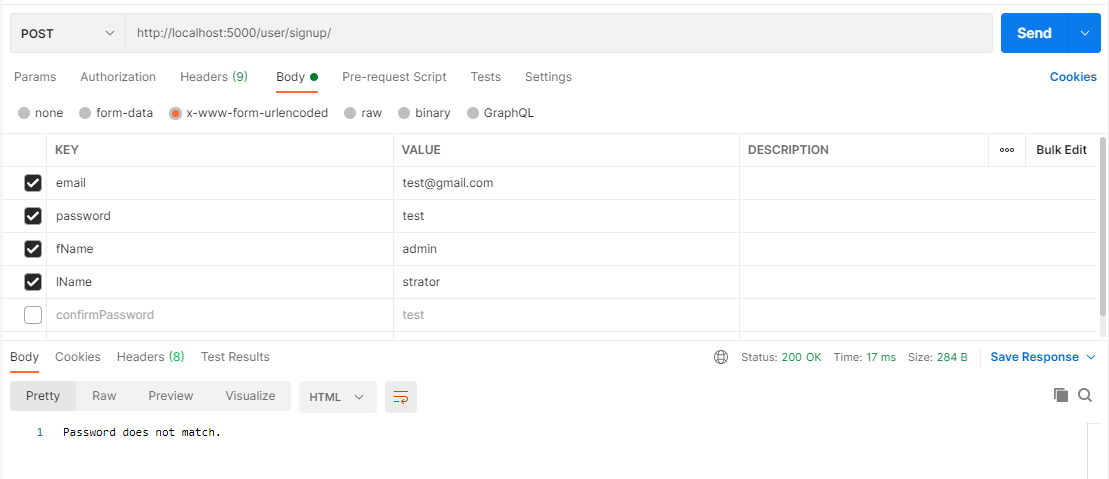
\includegraphics[scale=0.45]{img/test-make-user-wrong-pass.png}
    \caption{Testing the backend using Postman}
    \label{fig1:post1}
\end{figure}

\section{Development Tools}During development of the project, I intended to use a few different tools. The use of these tools would allow for different ways of keeping track of the progress of the development of the application. These tools include GitHub and Postman as mentioned above in the testing section.

\subsection{GitHub}GitHub is a service that I and others have been using for college since the beginning. It is a tool that I am very familiar with due to using it for not only this project, but many others throughout the years. It is a very important tool to use in development as it keeps track of the state of the project. The project is stored inside of a repository and every time a change is pushed, the repository is updated to the latest version, but it also keeps track of the previous commits. These can be helpful if the developer wishes to rollback to an earlier version of the program in case code with a mistake was pushed to the repository. It is also very helpful in group projects, making sharing work amongst group members easy through branching, or raising issues that need to be fixed.

\subsection{Yarn}Another tool I plan to use in the development of this app is a part of the node package manager (npm). Yarn is another just like npm and is installed via npm. While npm does have the same capabilities as yarn, yarn makes sure that the developer only has the one package and not multiple copies of it with multiple version of it. The advantage of using an external package manager from npm, is that it allows the developer to keep the dependencies local only to that single project. This eliminates the risk of technologies or different versions of the same technologies from clashing and causing errors / bugs during development.

\section{Research}During the creation of the project, my main form of research was based on practicality. This involved writing code alongside tutorials or following documentation to get an idea as to how the technology worked. However there were instances where I used theoretical research such as when picking a color scheme for the application, as that involves psychological aspects, like needing to grab the users attention but also not make a very bright or clashing palette that would dissuade them from using the application. For this instance I had to research for color palettes that meshed well and also fit into the them of the web application.

\chapter{Technology Review}
\section{Technology Review Introduction}
The objective of this project is to provide a scalable, intuitive and an easy to use forum web application, while using it as a learning experience to grow my skill set in the development of web applications. This chapter will give insight and detailed explanations regarding the steps taken to choose the technologies for the development of this project through research. Using the research of the different technologies, comparisons will be made between the technologies to justify reasoning behind choosing a technology for developing the application. Different criteria will also be used to judge the technologies. The criteria will pertain to things such as, ease of use, appropriateness to the application proposed, security, ease of testing and scalability. The technologies used should also allow for the creation of an easily manageable application to integrate new features alongside solid documentation. At the same time it should also be challenging enough to allow for growth and expansion of knowledge and skills during development.

This chapter will be split into subsections where I will look into the technologies that cover different domains, such as different stack technologies, databases, version control, authentication and hosting.

\subsection{Stack Technologies}
A technological stack is a combination of programming languages and underlying software that is used for the creation of web or mobile applications. The combination of these technologies is very important as they form a solid framework to work with. If the combination between these technologies is poor, then there may be some underlying issues that can occur between the front-end and the back-end. Luckily the majority of the technologies in stacks are versatile and the different components that make up that stack are compatible, and if they are not, someone has most likely developed a package that solves the compatibility problems between the technologies. The main two stack technologies I looked at were the MERN stack which consists of MongoDB, Express.js, React and Node.js. Alongside the MEAN stack which consists of the same technologies except React is replace with Angular. The only change between these two stacks is the front-end framework technology.

\subsubsection{Server Side - Node.js, Express.js}
The mutual technologies associated with both stacks are MongoDB, which is a database used for storing the information that is associated with the application and, Express.js and Node.js which are components closely linked to each other as Express is a web framework that is used to enhance the function of Node.js \cite{mozillaNode}. Node.js is a cross-platform runtime environment that allows for the development of web servers and the server side utilities. It is created to run directly on any Operating System (OS) making its features accessible on any machine. Another feature is that it allows the developer to access the node package manager which contains a vast array of packages to aid in the development of web applications. It is supported by the majority of hosting services and uses JavaScript as its programming language. The vast amount of documentation available for it allows developers to get a server that listens for HTTP requests up and running very quickly.

Express.js is a web framework that runs underneath Node.js \cite{express}. It provides the ability to create handles on different HTTP requests for different URL paths/routes. URL routes are the locations of where the resources to a web page are located. For example, a simple route could be written like this: "https://www.mywebsite.com/pictures/image.png". In this case the route would return a response of an image that is located in the pictures resource folder of the domain. Express allows for a minimalist approach to creating these types of routes, whether the user of the application wants to request a resource from that route i.e. the image, or whether they wish to create an account and they submit data to a route that is defined by express. When data is pushed to that route, Express receives that data from the Node.js server, Express can then be used to handle to handle the data and send a response back to the Node.js server. The responses returned can vary based on the routes defined. One route could be defined to register a user, Express would get the data from the Node.js server, run it through the logic required to create a user and return a response. This allows for streamlined development of the back-end portion of a stack, with these two technologies working in tandem. Figure [\ref{fig2:node}] is a simple diagram showing the relationship between a Node.js server and the Express.js web framework. The middleware is the representation of express handling the data, like registering the user and sending it to the database, and then sending back a response back to the client, whether it was successful or not. The integration between these two technologies also satisfies some of criteria mentioned earlier, such as ease of use because of the thorough documentation and the widespread use of technology. It also satisfies the criteria for both ease of testing and scalability. As mentioned earlier, programs such as Postman would allow for automated testing of routes, and with the technology being able to run on all machines it is in turn scalable.

\begin{figure}
    \centering
    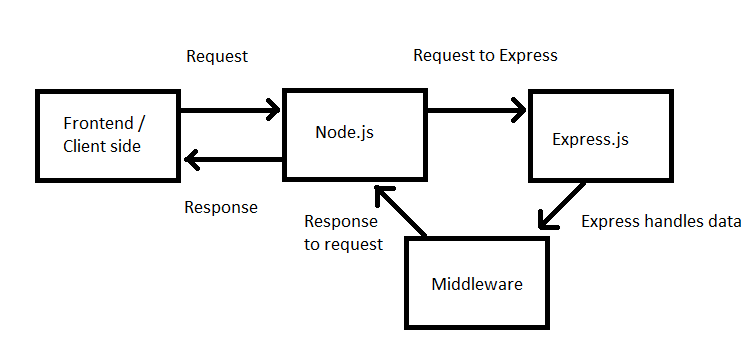
\includegraphics[scale=0.7]{img/node-express.png}
    \caption{Relationship between Node.js server and Express.js web framework}
    \label{fig2:node}
\end{figure}

\subsubsection{Front-End - React vs. Angular}
Both React and Angular are commonly used to develop robust front-end applications, the main difference regarding both of these programming languages is, React is a library and Angular is a framework, and choice between the two, should be decided based on the requirements of the project. Both of these technologies are also well established and maintained. React is maintained and developed by Facebook, while Angular is maintained and developed by Google. This provides solid documentation for both of these technologies. There is one main similarity between the two languages, but a lot more differences. Lets take a look at the similarity first.

Both of these technologies use components as a base to create single page web or mobile applications. Components are scripts that allow for seamless changes in the UI and the render shown to the user. When a user on the web page wishes to go to another page, components give the illusion that they are changing pages, when in fact they are just replacing the current component with another one. This significantly decreases load time since they never actually reroute from the main page.

Differences between these two technologies begin with the language. React uses the JavaScript library and since it not a complete framework it requires the installation of a variety of packages to achieve data-binding and component based routing. These include packages like React-Redux and React-Router-Dom. While this may seem like a disadvantage to using React, it allows the developer to customise and install only the libraries needed for development. Saving space and decrease complications between a whole suite of packages that may come built with a framework. The advantage of having only relevant libraries pertaining to the project also decreases set up times and load times. The developer may also use external package managers such as Yarn, to manage the dependencies and packages, this also gives the developer full control over the versions of the technologies used. React is also great in terms of performance as it uses a virtual DOM, which is generated by the server. This reduces load on the browser when the web application is being rendered, it achieves this by keeping the UI in memory and syncing it with the actual DOM. So in the event of a state change, the DOM only changes the elements where the state changed, reducing load times significantly. This is method is also called reconciliation \cite{reactDom}. A caveat of React however is state management if no external libraries are added. If no external libraries such as React-Redux, which is most popular and well documented. React applications would force the developer to state the state of each component in multiple parts of the component. If the developer wished to pass these states from one component to another, it would have to be done manually each time. This would be a very time consuming process. However, react-redux eliminates this problem through the use of a global store, more about the details of this library further down this chapter.

Angular on the other hand is a full framework. This means that it usually does not require the addition of external libraries to access features like data-binding and component-based routing. This limits the customisation of libraries and the developer is forced to use the suite of provided libraries. Unlike React, Angular uses TypeScript as the language. The main advantage of TypeScript over JavaScript, is TypeScript can compile down to JavaScript allowing all browsers to interpret the code without problems. However this technology does have a significantly steeper learning curve compared to regular JavaScript. Performance with Angular also tends to be slower, due to watchers. Watchers overlook data-binding and they run continously looking for changes in the state. As the application gets more complex the amount of watchers between different components may burden the browser, causing slower load times. Since Angular is a framework, the state is handled through inputs in the components. This means the state is always being handled and no real manual passing of the state from component to component is necessary.

Between these two stacks, the MERN stack was ultimately chosen. Reasoning behind this decision was the advantage React had over Angular when it came to making complex web applications. The versatility of React would allow for the precise management of packages, which are only relevant to the project at the moment of iteration. This would help with keeping the size of the application smaller, keeping load times fast. The requirement of the project is to create a forum web application. Forums can start out simple, but over continuous iterations and feature additions, the versatility of React would be a bigger benefit in the long term, over Angular \cite{reactangular}.

\begin{figure}
    \centering
    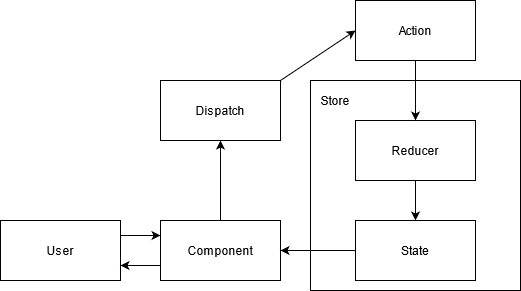
\includegraphics[scale=0.7]{img/redux.png}
    \caption{Redux state management flow}
    \label{fig3:redux}
\end{figure}

\section{React-Redux}
React-Redux is a state management library, that is used by the majority of applications that use React. Without redux, tracking the state of every component in the application would create a heavy burden on the developer as more features get implemented. This is because the developer would have to keep track of the state of every component. If the developer wished to pass the state of a component to another not located in the same hierarchy, a manual store would have to be created and the state would have to passed down through the components. If the application is small in size then, this style of state management is more that feasible, however for applications with the possibility of long term development and an increase of complexity during development, Redux is a worthwhile library to have integrated into the project \cite{reactredux}. 

Redux manages the state of the application through three features. They are actions, reducers and store. When the user interacts with a component, and causes a change in the state. An action is dispatched. The action sends the data to the reducer. The reducer then sets the state of the application to the new state that was just dispatched. The store then keeps the current state until another action that changes the state is dispatched. Keeping the state stored globally in a single area, avoids the issues of having to manage a variety of different states for different components. Redux also comes with an increase in performance, when it comes to rendering components. The code is well optimised and have a single store, removes the need for constant re-rendering of components, as redux keeps track of the data and wont re-render if the data has not changed. Redux also adds structure to the project, by having all the actions and reducers separated, allowing the developer to create a seamless workflow between components, actions and reducers. If the project size and complexity grows, having a uniform structure that can manage states of different components, would allow for faster and more efficient development of the features.

\section{Database - MongoDB}
With the project being a MERN stack, MongoDB was an obvious choice for the database. There is a choice between Mongo databases. There is a desktop version that is run locally on the developers machine or a server OS. However there is also an online version called Mongo Atlas. Mongo Atlas was the chosen platform for storing information pertaining to the application. Reasoning includes that, the set up is very easy and linking the atlas API to the back-end of the application is well documented. Mongo Atlas also makes it very easy to set up clusters, which house collections. The collections are where the data is stored, and the place accessed when retrieving or submitting data to the database. The database also has some extra features, like managing the IP addresses that are allowed to make requests from the database, it also allows for the deletion of or editing of the contents of the stored data through an easy to use UI, making it useful when testing features such as sending get requests to the database. Figure [\ref{fig4:mongo}] displays the way Mongo Atlas stores and shows data when accessing the collections. Another positive of the Mongo Atlas database is that the data is stored in JSON format.

\begin{figure}
    \centering
    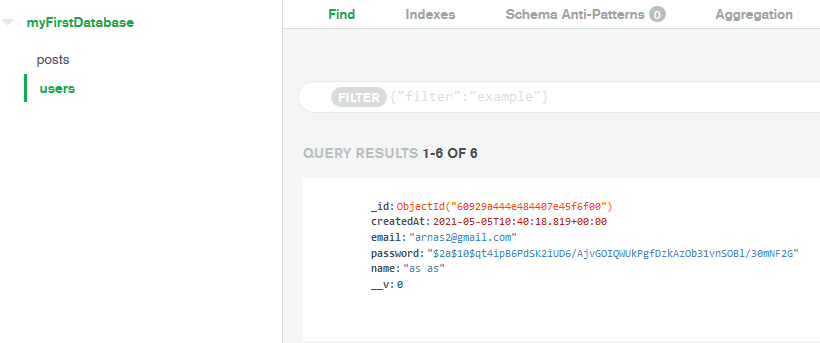
\includegraphics[scale=0.7]{img/database.png}
    \caption{Mongo Atlas Collections}
    \label{fig4:mongo}
\end{figure}

\section{Authentication}
Authentication is a crucial component of applications that deal with the handling and storage of user data. It is a necessary feature that ensures users are allowed to access information only they are privy too, and also for keeping the information secure. This application will use two different libraries for encrypting the user details and determining whether a user has permissions to perform certain actions based on who they are. The two libraries are bcrypt and jsonwebtoken. Bcrypt is a library that allows for an easy way to encrypt and decrypt data. It uses a hashing algorithm and salting to hash data. Salting is an extra input added to the hash to prevent the data from being decrypted via rainbow tables. Salting input is mainly a secret key that the developer of the application creates. This secret key is then stored inside of an environment variable so that only the developer has access to it. The jsonwebtoken library will be useful in determining the user and giving them permissions to execute certain actions, by assigning them a unique token on registration or when they login.

\subsection{Hosting}
Hosting is a great way of providing access to the developed application through the internet. There is a multitude of different hosting providers that can host web applications for free. The two options that were considered were Heroku + Netlify working in tandem and Firebase \cite{heroku}\cite{firebase}. Both of these hosting providers give a free service. Firebase is a platform set up by Google and helps in the development of applications by providing features such as authentication and database storage. While these features are certainly helpful, using a MERN stack would not be able to utilise the full features of the hosting provider. Without being to utilise the full capability of a hosting provider, it was decided to use Heroku. Heroku has detailed documentation and is also very popular for hosting full stack applications and restful applications aswell. I have also had previous experience with hosting on Heroku, but I did not have any experience with Netlify. Netlify allows the developer to host the front end of the application just by creating a build of the client side and then uploading it to the website. While this does require the use of two different websites, it also keeps the client side separated from the server side. This organisation separation could prove useful in the long term, so the decision was made to use Heroku alongside Netlify to host the application.

\subsection{Version Control - GitHub}
GitHub was a major part of the development process. While it did not contribute to the development of the project, it allowed for the tracking of progress through the life cycle of the application. It was also a good way to back up the progress that was made on the application, just in case something went wrong, there would a version of the application to fall back on, not losing any progress.

\chapter{System Design}
\section{System Design Introduction}
This chapter will explain the process behind the development of the web application. It will also delve into the code that runs the application and provide explanations the functionalities the code adds and how it works. When designing the system that has to be implemented, it is important to determine the structure of the project and have a baseline to work from. Once the baseline of the features and functionalities was determined, I began researching into to the different technologies that would be used, and got a little handle on the technologies usage. I followed the official documentation and guides that get developers started in using the technology. During the process of development, keeping the files in a structured manner or code neat using best practices, whether it was indentation or function declarations was vital. Giving a sensible structure to the project allowed for navigating between files and also linking files to each other easy, it was also easier to figure out which components work together by keeping structure. There was real value in keeping the code base consistent with the best practices and the file structure organised, and the hope was to keep it consistent between the server side code and the front end code. 

Being a solo developer for this project did serve a few problems, however. It did not allow me communicate my ideas to anybody else, but I also did not have anyone to critique my code and suggest improvements that could be made. Another difficulty that I encountered was that even though I had kept the file structure of the application consistent and organised, it still got difficult having to manage both the front-end and the back-end logic of the application simultaneously. Even though I worked on the back-end first, creating routes and the logic for handling of data, then moving onto the front-end portion. There were times when the code would get confusing having to change states of the front-end while simultaneously passing data to the back-end to get responses. Being in a group would have made this an easier process to deal with, as the tasks could be decided amongst each other i.e. one developer would be responsible for the front end while another team member would be responsible for the back end logic. But, there were also benefits to developing this application solo, the main one was that it did allow me to get a great grasp on the technologies, due to being responsible for both front-end and back-end. By working solo on this project my understanding of web applications increased greatly, and helped me accomplish my main objective for this project, which was to learn and improve my skill set as a developer for creating web applications. The main topics to cover in the design of the application will be linked to these subsections: Front-End, Back-End, Authentication, Hosting and UI Design.

\begin{figure}
    \centering
    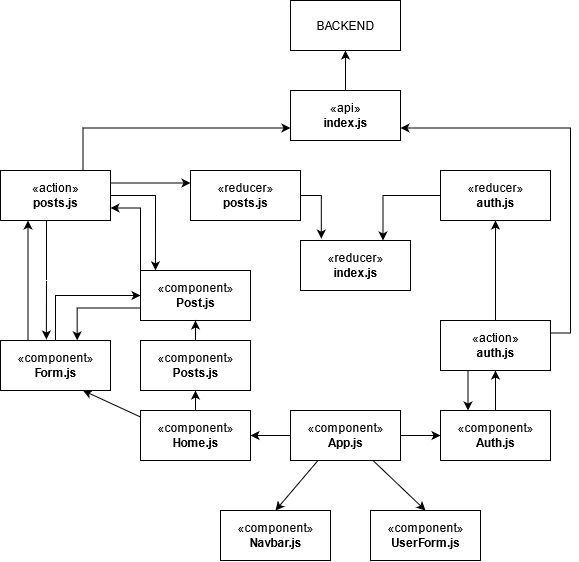
\includegraphics[scale=0.7]{img/UML.png}
    \caption{Architecture of the front-end}
    \label{fig5:frontend}
\end{figure}

\subsection{Front-End}
The client side, or the front end of the application utilises React and React-Redux alongside libraries like axios to make requests to the back end. Figure [\ref{fig5:frontend}] down below, displays the whole system architecture and the interactions between all the components alongside the react redux features, which are actions, reducers and the store. When I first began working on this project, I had to relearn a lot of the features of the React library which I had not used in over 2 years. Alongside relearning React, I had to learn how to use react-redux to manage the state of the application. This proved to be difficult in the beginning, with how components interact with the dispatch actions and the reducers to manage the state of the store. However, because of the abundance of documentation and available tutorial, this allowed me to get up and running pretty swiftly. The incorporation of react-redux was a good decision, as in the long-term when I added more components and had to manage the different states of these components. React-redux added structure to the code base. It allowed me to manage the state of components that simultaneously that did not have any links to each other. As an example in figure [\ref{fig5:frontend}], I had state management for Posts and Auth components. These two components are not linked in any way except through the reducer called index.js which combines them. By combining them, they were both stored in the same global store, which allowed me access the state of both of these components from different parts of the application. Lets take a look as to how this sort of state management is achieved.

\begin{minted}{js}
Auth.js

<form className={classes.form} onSubmit={handleSubmit}>
    <Grid xs={12} md={12}>
        <TextField name="email" label="Email Address" 
        onChange={handleChange}
        type="email" 
        required 
        autoFocus 
        fullWidth/>
    </Grid>
    
    ... Other fields
    
    <Button className={classes.qButton} type="submit" variant="contained"
    color="secondary">
            { signedUp ? 'Sign Up' : 'Sign In'}
    </Button>
</form>
\end{minted}

The first task we must do is create a way to submit data. In this case I created a form that has a name, a label and a hook that gets called when the submit button at the end of the form is called. This is what the logic in the hook is like:

\begin{minted}{js}
Auth.js - components/Authentication

// functions to execute when user submits
const handleSubmit = (e) => { 
    e.preventDefault();
    if(signedUp) {
        dispatch(signup(formData, history));
    } else {
        dispatch(signin(formData, history));
    }
};   
\end{minted}

This hook, creates a dispatch to the auth.js file located in the actions folder in the hierarchy of the application, which has a function that handles the formData and the history of the application. The history is a feature of react-router-dom which is used to redirect the user to different components. The form data which is submitted, is just the data the user typed in to create an account in this case.

\begin{minted}{js}
auth.js - actions/

export const signup = (formData, history) => async (dispatch) => {
  try {
      const { data } = await api.signUp(formData);
      dispatch({ type: "AUTH", data });
      history.push('/');
      window.location.reload();
    } catch (error) {
      console.log(error);
    }
};
\end{minted}

Going line by line, this is what occurs once the action is dispatched from the component. We have defined and exported a function called sign-up, that takes in formData, and the history of the application. Using redux-thunk, which allows redux to create asynchronous dispatches, we call the signup api function and pass it the data so that it can be sent to the back-end and a user can be created. This is what the request looks like:

\begin{minted}{js}
index.js - api

export const signUp = (formData) => instance.post('/user/signup', formData);
\end{minted}

Going back to the snippet above, a variable is created and stores the data from the api response. We then dispatch again this time to the reducer, which defines how to store the state of the data globally in the application. we then push the user to the home page after registration and reload the application window. Below is the code snippet of how the reducer stores and changes the state globally based on the data it receives.

\begin{minted}{js}
auth.js - reducers/

const auth = (state = {data: null}, action) => {
    switch (action.type) {
        case 'AUTH':
            // add the user to localStorage to handle the state of the shown website
            localStorage.setItem('profile', JSON.stringify({ ...action?.data }));
            return { ...state, data: action?.data };
        case 'LOGOUT':
            // remove the user information from localStorage
            localStorage.clear();
            return { ...state, data: null};
        case 'DELETE_USER':
            const { user } = action.payload;
            localStorage.clear();
            return user;
        default:
            return state;
    }
}

export default auth;
\end{minted}

When the dispatch was made to the reducer, I added parameters to the dispatch, they were the type and the data, it was in this line of code.

\begin{minted}{js}
auth.js - actions/

dispatch({ type: "AUTH", data });
\end{minted}

By giving our dispatch the type, this is what determines the type of action executed when storing the state globally and what to return. Since the type we passed was "AUTH", in the switch, we will enter the "AUTH" case. The first thing that occurs is we set give the user a JSON web token which will be gone over in detail in the authentication section. Then we return the newly set state, which can be used accessed from other components. In this case, the new state is used to check whether some is logged in or not, and based on this the component decides what the user is allowed to see. To get the state to be able to do such actions only one line of code is needed. 

\begin{minted}{js}
NavBar.js - components/Navbar

const [user, setUser] = useState(JSON.parse(localStorage.getItem('profile')));
\end{minted}

By getting the state that is stored we can use it in cases like these:

\begin{minted}{js}
NavBar.js - components/Navbar

<Toolbar>
    {/* Ternary operation to display different objects in the toolbar based on 
    whether user is logged in or not */}
    { user ? (
        <div>
            <Button className={classes.qButton} component={Link} 
            to="/userdetails">
            Profile
            </Button>
            <Button className={classes.qButton} onClick={logOut}>
            Logout
            </Button>
        </div>
    ) : (
        <div>
            <Button component={Link} to="/auth" 
            className={classes.qButton}>
            Sign In
            </Button>
        </div>
    )}
</Toolbar>
\end{minted}

By checking if there is something in the user state, ternary operators can be used to render different aspects of components. In the case above, it checks for a user, if the user state is returns as logged in it displays a Profile button and a Logout button, else, It just displays a button called Sign in, which redirects the user back to the Auth.js component. Similar logic is applied when creating and handling forum posts in another component.  Figure [\ref{fig6:redux-flow}] down below showcases what the flow of data from the submission form to the render of the data in the post component looks like.

\begin{figure}
    \centering
    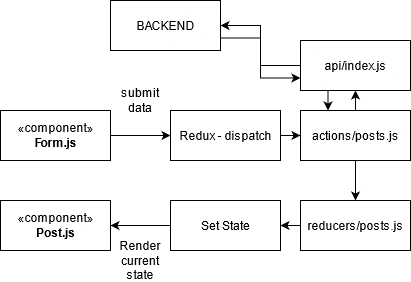
\includegraphics[scale=0.7]{img/redux-flow.png}
    \caption{Redux flow for Post components}
    \label{fig6:redux-flow}
\end{figure}

\section{Back-End}
The back-end is responsible for the storage, processing and handling of the data the web application utilises. The first step I took in the development of the database, was to create a structure that would keep the separate components that made up the back-end separated. These components were the main server file itself, a folder that stored the routing for the back end requests, the models folder, which defined a schema by which to store information in the database, a middleware folder which would be used to verify users via the backend and send back responses as to whether they have permissions for certain features or not, and finally the controllers folder. The controller scripts were responsible for the handling and processing of the data. The back-end just like the front-end also utilised a variety of different libraries such as mongoose to allow communication between the Node.js server and the MongoDB database. CORS to allow users from different domain to gain access and be able to load resources. Figure [\ref{fig7:backend}] displays the basic interaction between the components that make up the back-end.
\begin{figure}
    \centering
    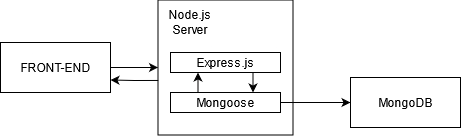
\includegraphics[scale=0.7]{img/back-end.png}
    \caption{Back-End Interactions}
    \label{fig7:backend}
\end{figure}
The second to developing the back-end was to create a server that can run locally and connect to the database. This was done by creating a server.js in the root directory and importing the necessary libraries like mongoose, express and cors. I followed the getting started tutorial on the Express.js website to get a quick skeleton server running \cite{express}. I then defined the model, which was a schema by which the MongoDB database would store objects. Here is an example of the Post Model.

\begin{minted}{js}
posts.js - models/

const mongoose = require("mongoose");
//const User = require("user");

// define Schema
const Schema = mongoose.Schema;

// create post model
const PostSchema = new Schema({
    title: String,
    message: String,
    name: String,
    user: String,
    file: String,
    likeCounter: {
        type: [String],
        default: [],
    },
    dislikeCounter: {
        type: [String],
        default: [],
    },
    createdAt: {
        default: Date.now(),
        type: Date
    },
    comments: {
        type: [String]
    }
});

const Post = mongoose.model("Post", PostSchema);
module.exports = Post;
\end{minted}

When I decided to implement the functionality to create a Post the schema allowed me to store the data in an organised way inside the database. The Post model is utilised by the script inside the controller. The controller uses data passed in from the front-end to populate or return the different fields inside a model that is stored in the database. This is an example of how I created a post and stored it in the database. Once a good structure is implemented in the back-end the process of adding new features does not change much except for the logic inside the functions. The first step is to define a route to send our requests to.

\begin{minted}{js}
posts.js - routes/

const express = require('express');
const router = express.Router();

const { createPosts } = require('../controllers/posts')

router.post('/', createPosts);

module.exports = router;
\end{minted}

When a request is sent to the defined route, we go to the controllers and execute the createPosts fucntion.

\begin{minted}{js}
posts.js - controllers/

const express = require('express');
const mongoose = require('mongoose');
const Post = require('../models/post.js');

// Create a new post
const createPosts = async (req, res) => {
    const post = req.body;

    // spread the data/params of the post and assign the token id to user
    const newPost = new Post({...post, user: req.userId});

    try {
        await newPost.save();
        res.status(201).json(newPost);
    } catch (error) {
        res.status(409).json(error);
    }
}
\end{minted}

Going line by line, we first declare our imports, and among them is the model. When the request is made to the routes, it brings us to createPosts function. The information inside the request gets stored inside a post variable. We then define another variable to store the a new Object with the data. Then entering the try catch block, we attempt to save the post to the database and if successful it return a status response otherwise it returns a response that an error occurred.

Just like the front-end, by having this structure in the back-end, it allowed me to have a consistent workflow, without having to do an entirely different process for the handling of each request.

\section{Authentication}
Authentication in this application was used as a way to verify whether the user was allowed to access certain features of the application through the use of JSON web tokens. I started by creating a function that would receive a web token when a user logged in, it would decode that token and compare it with the users id inside the database. If there was a match the function would permit the execution of certain actions. This function was exported and then if put in as a parameter to certain route requests, the user would be authenticated. The authentication was connected through three separate components. They were the auth.js file, routes.js and then the api.js scripts located in the front-end by using hooks.

In the application authentication would begin on sign in.

\begin{minted}{js}
NavBar.js - components/NavBar

const [user, setUser] = useState(JSON.parse(localStorage.getItem('profile')));
\end{minted}

Using states when a user is created we can store the data located in local storage and set the users state to the data. Then when a user makes a request from the front-end, the request goes through the api.js script.

\begin{minted}{js}
api.js - api/

instance.interceptors.request.use((req) => {
    if(localStorage.getItem('profile')) {
        req.headers.Authorization = `Bearer \${JSON.parse(localStorage.getItem('profile')).token}`;}

    return req;
});
\end{minted}

Using a method of axios called interceptors, we can intercept a request, and then get the json token that is associated to the user and store it in the Authorization header. This is called the bearer token. Before the request is fully executed we send the token and run it through middleware in the back-end. This is what the middleware script is composed of.

\begin{minted}{js}
auth.js - middleware/

const auth = async (req, res, next) => {
    try {
        // get the authorization header from the request, which is the bearer token
        const token = req.headers.authorization.split(" ")[1];

        if(token == undefined) {
          console.log({message: "User not logged in."});
        }

        let decodedData;
        
        // decode the token using the secret key
        decodedData = jwt.verify(token, process.env.SECRET_KEY);
        // set the request header userId to the decoded token id
        req.userId = decodedData?.id;  
    
        // executed the task after decoding
        next();
      } catch (error) {
        console.log(error);
      }
};
\end{minted}

When the request is made, we store the token by accessing the authorization header, if there is no token we return a message saying the user is not logged in. If there is a token we use jsonwebtokens verify function on it and pass in the secret key. If this returns true the user id is set to the token id and the user is allowed to go through with the request.

\section{Hosting}
The project is hosted through two different providers. The back-end and the front-end are hosted separately. The back-end is hosted on heroku and the front-end is hosted through netlify. Heroku allowed for an easy way to run the server side files by adding them to heroku git repository and the set up was very easy. Thanks to the documentation that is provided when generating a new heroku application. Netlify allowed me to host the client side of the application in a very easy manner. All I had to do was build the project and then drag and drop the build contents to Netlify. My reasons for separating the front-end and back-end  when hosting is for ease of access. If I need to work on the back-end then I can just push my changes to the heroku repository and vice versa, if I needed to change some front-end features, I could just create a new build of the front-end and replace the existing one, without ever needing to shut down the website. As the two components are hosted separately.

\section{User Interfaces}
For this project I used a simple design for the UI as I did not want to clutter the web site with unnecessary details. I also used a simple colour scheme between four colours. I also used a library called Material-UI to customise and design the layout of the UI. Material was very handy in the way that it allowed me to created custom styling using hooks and importing them. Below are the different web pages that are in the application.

\newpage
\begin{figure}
    \centering
    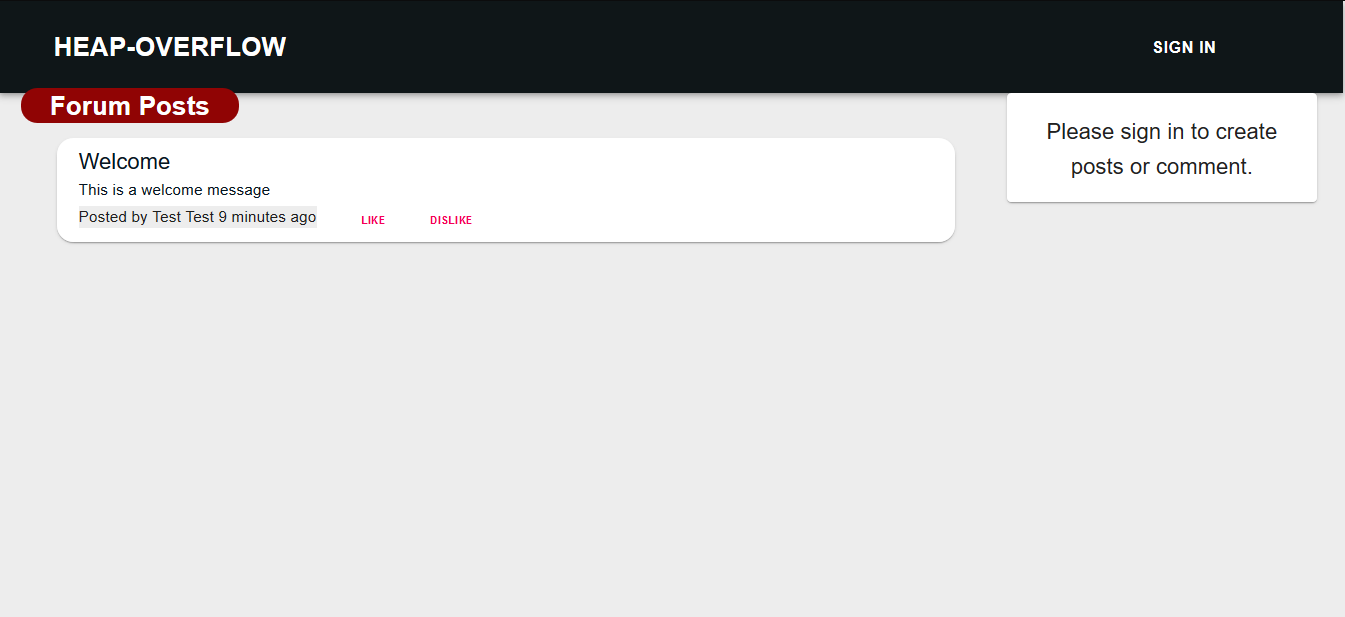
\includegraphics[scale=0.4]{img/UI/logged-out.png}
    \caption{Home Page}
    \label{fig8.1:home}
\end{figure}
\begin{figure}
    \centering
    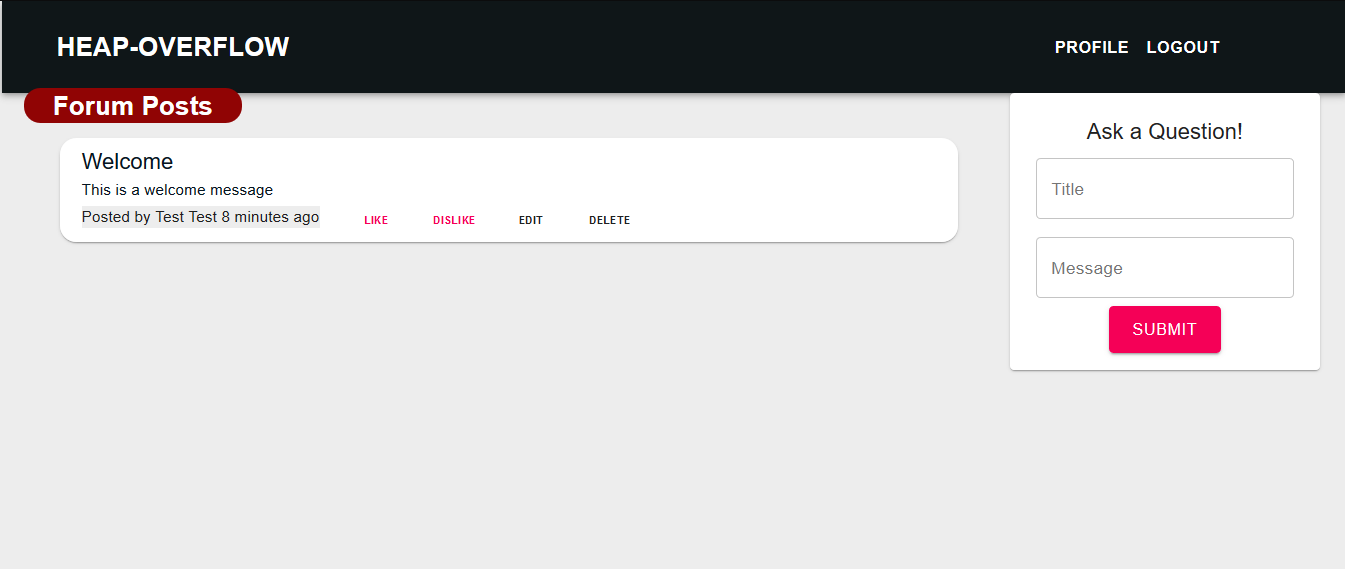
\includegraphics[scale=0.4]{img/UI/welcome.png}
    \caption{Logged in home page}
    \label{fig8.2:welcome}
\end{figure}
\begin{figure}
    \centering
    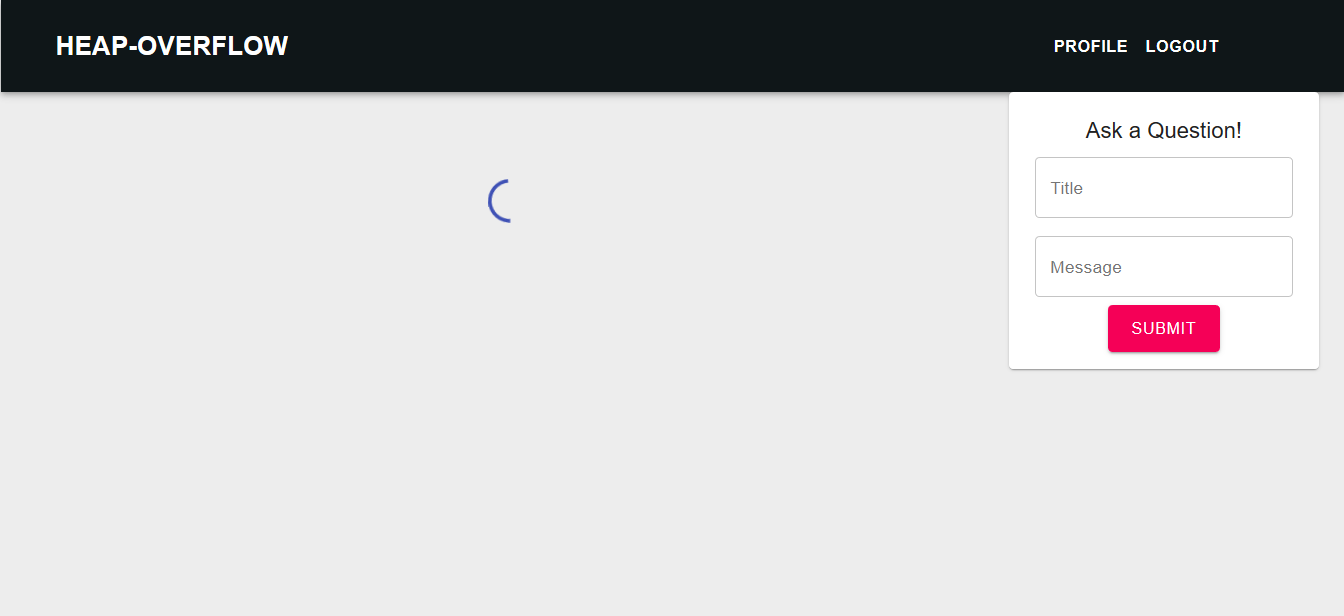
\includegraphics[scale=0.4]{img/UI/no-posts.png}
    \caption{Loading posts}
    \label{fig8.3:loadposts}
\end{figure}
\begin{figure}
    \centering
    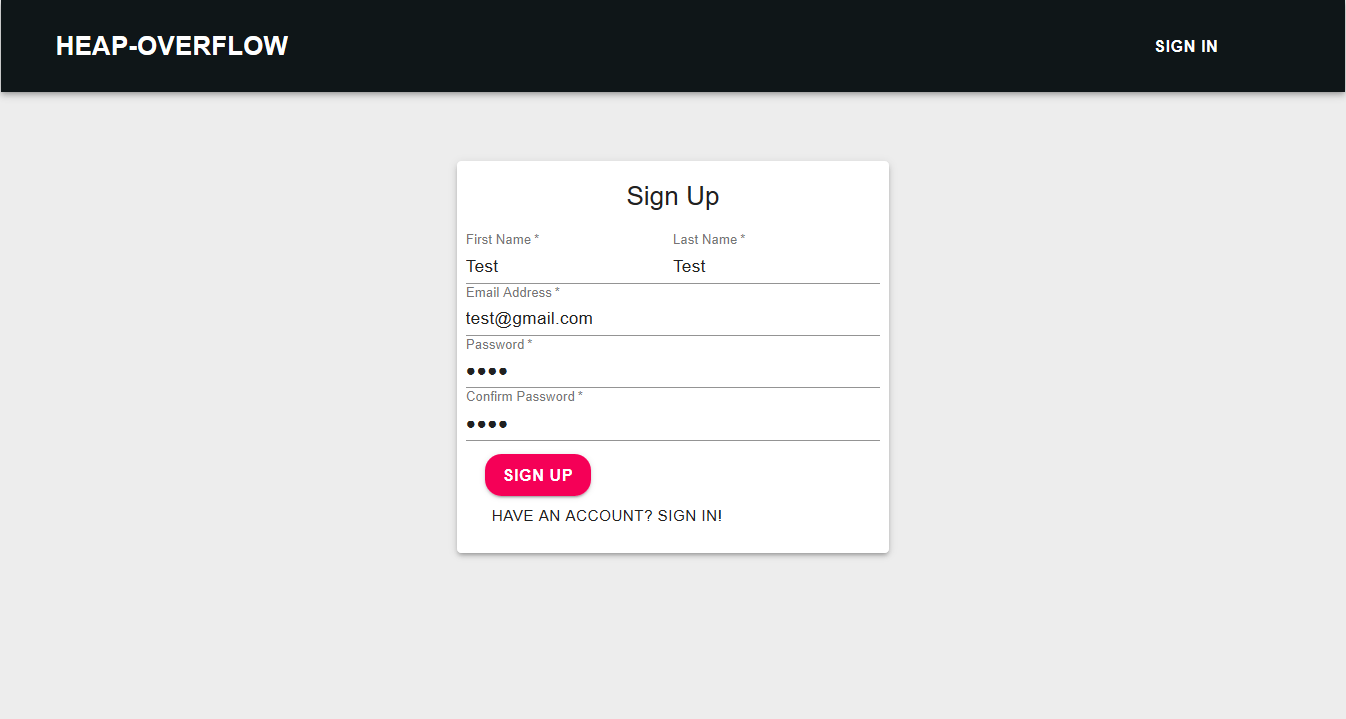
\includegraphics[scale=0.4]{img/UI/signup.png}
    \caption{Sign Up Form}
    \label{fig8.4:signup}
\end{figure}
\begin{figure}
    \centering
    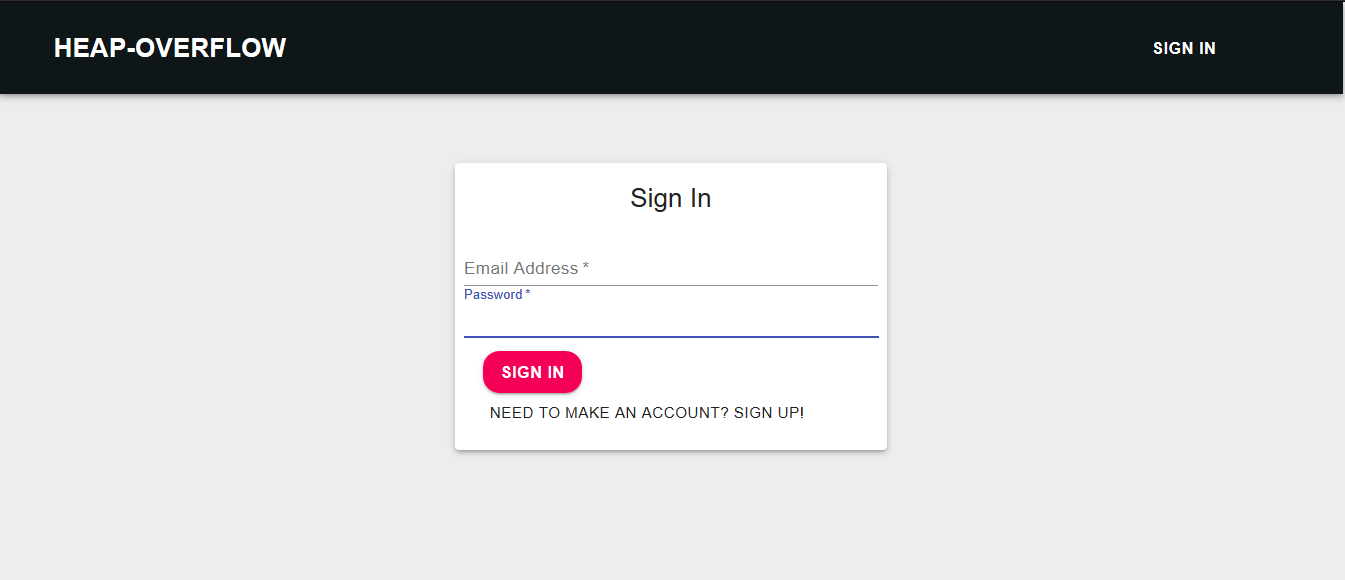
\includegraphics[scale=0.4]{img/UI/signin.png}
    \caption{Sign In Form}
    \label{fig8.5:signin}
\end{figure}

\begin{figure}
    \centering
    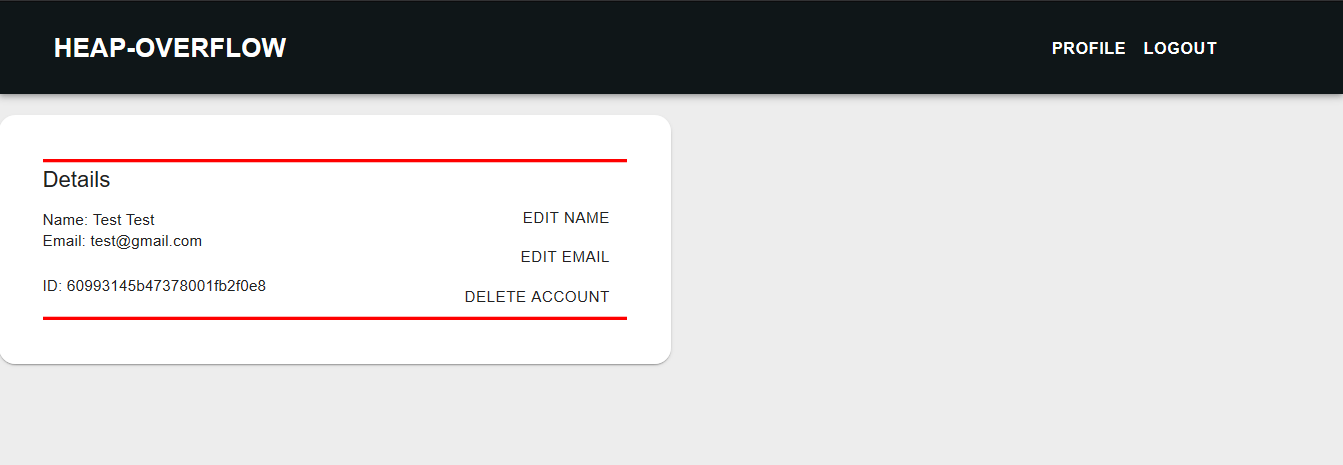
\includegraphics[scale=0.4]{img/UI/details.png}
    \caption{User Details}
    \label{fig8.6:details}
\end{figure}


\chapter{System Evaluation}
The objective when designing this application was to use it a learning experience and an avenue of learning to improve my skill set when it came to developing web applications. I also wanted to create a project that I would be able to work on in the long term, as technologies get updated, or I come up with new features to add to the project. To evaluate the system I tested it using a variety of way, these tests include using Postman to test the routing for the back end of the application and using google chrome built-in lighthouse tester to give me feedback on the performance of my application.

\section{Testing the Back-End}
To test the back-end of the application I used Postman. Postman is a program that allows developers to send all the available HTTP requests and receive responses. When I initially began work on the server side functionalities and I needed to test the responses and actions of the functions when data was sent to them. I used Postman as my primary tool. Using Postman made the work more efficient when it came to debugging problems, as I would not need to work about setting up the front-end before being able to see if the functionalities worked. I layed out objectives that had to be met, whether they were simple or not, such as:
\begin{itemize}
    \item Ensure a request can be sent to the desired route.
    \item Ensure the correct response is returned on faulty input.
    \item Ensure the correct response is returned on valid input.
    \item Ensure functions correctly execute when a request is sent.
\end{itemize}

\begin{figure}
    \centering
    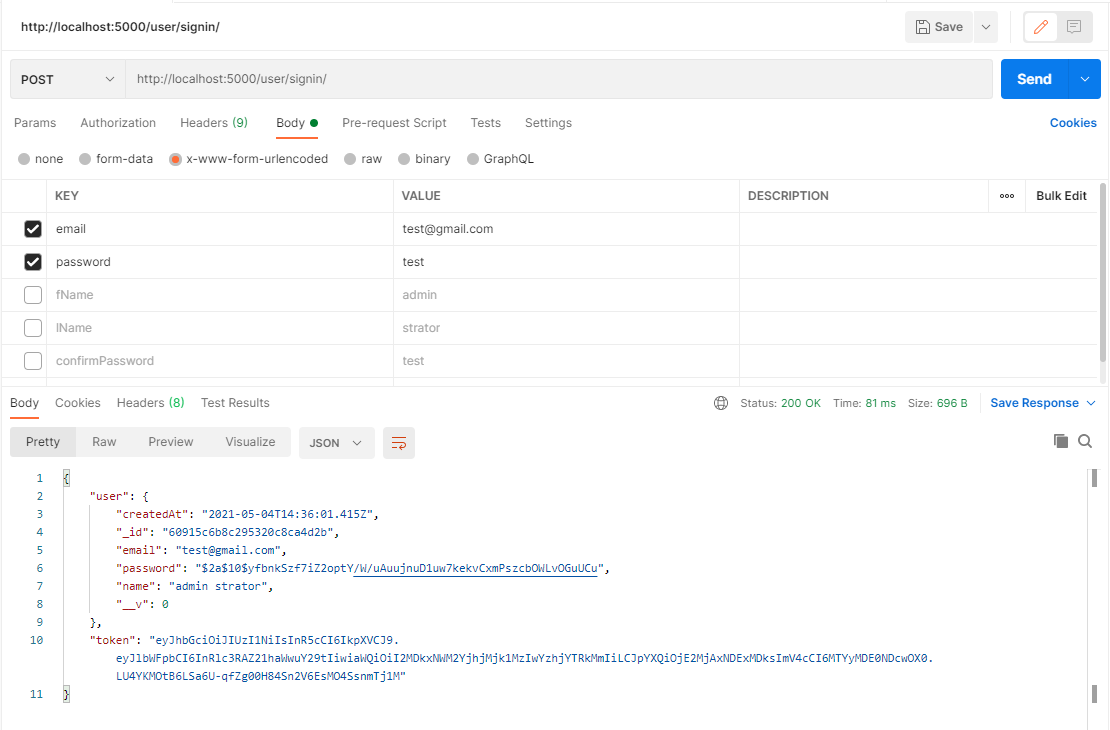
\includegraphics[scale=0.5]{img/Postman/login-success.png}
    \caption{Successful Login Response}
    \label{fig9.1:loginsuccess}
\end{figure}

\begin{figure}
    \centering
    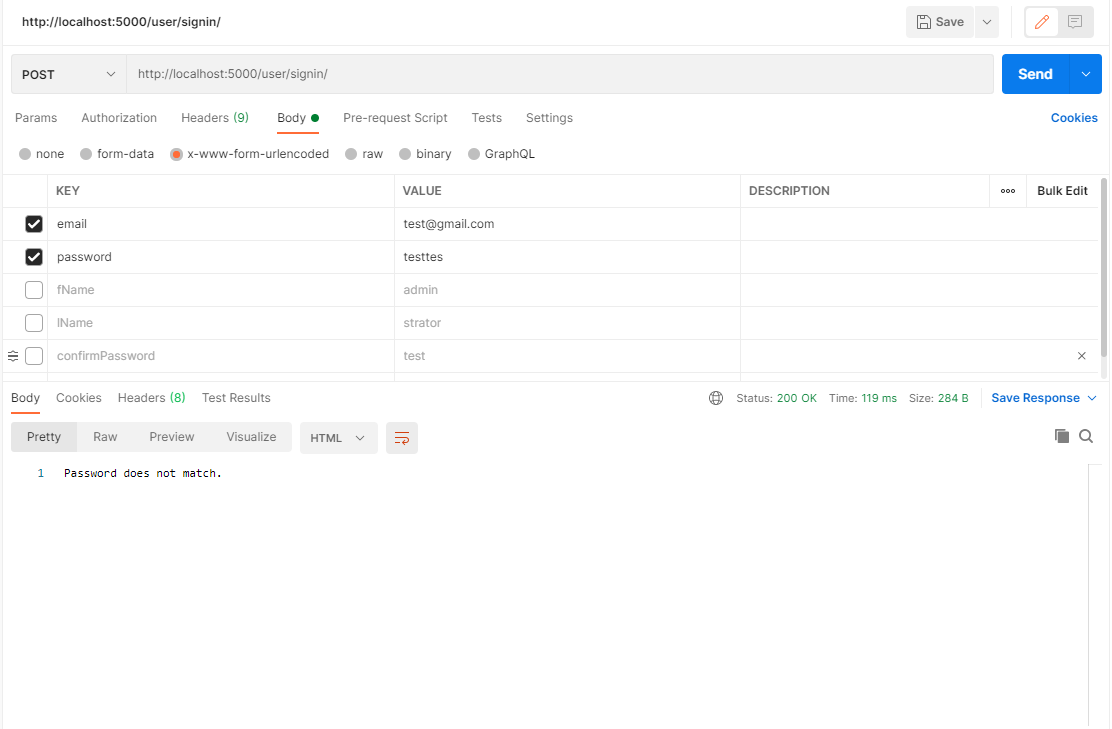
\includegraphics[scale=0.4]{img/Postman/login-bad-password.png}
    \caption{Wrong Password Response}
    \label{fig9.2:wrongpass}
\end{figure}

\begin{figure}
    \centering
    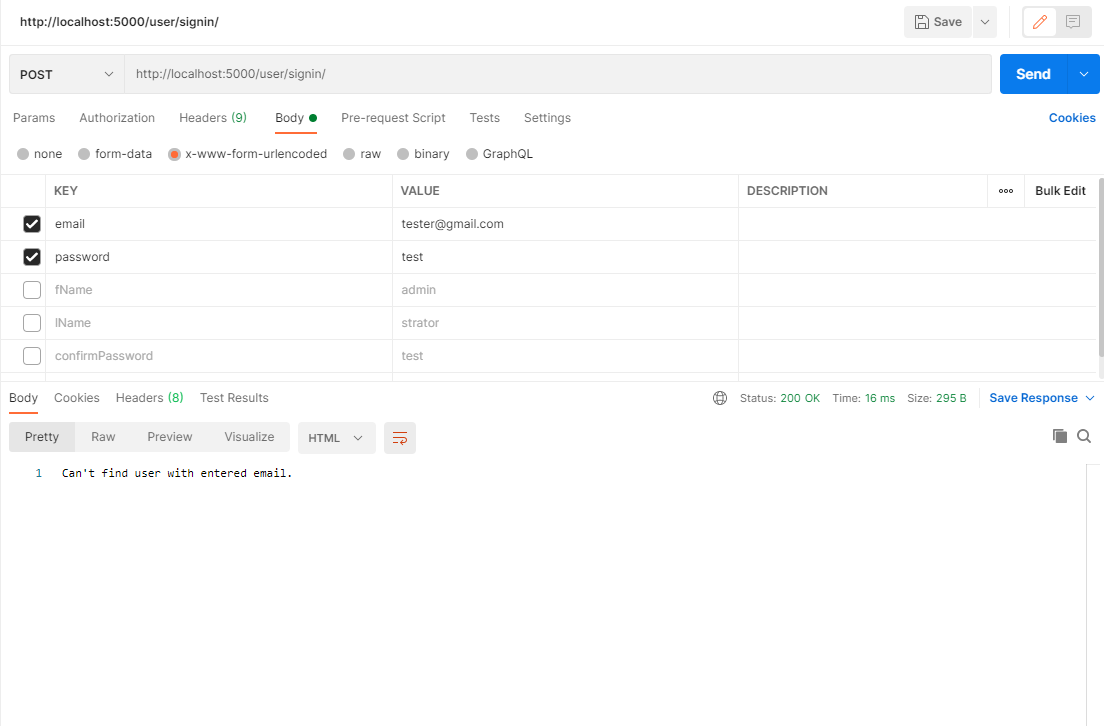
\includegraphics[scale=0.4]{img/Postman/login-bad-email.png}
    \caption{Wrong Email Response}
    \label{fig9.3:wrongemail}
\end{figure}

\section{Testing the Front-End}
The front-end tests were done in a similar manner to the back-end. While I did not use Postman or other external testing tools. I tested the front-end functionalities during implementation after the implementation of the features was finished. This also involved laying out objectives and benchmarks to which I tested the features against. Except this time I split the front-end into different sections that needed to be tested.
These sections included testing the Authentication features, User Interface features and the handling of data.

\subsection{Testing Authentication}
By testing the authentication feature of the application, I was also testing the user sign in and sign up functionality. These three components are linked together, as without authentication when creating an account or signing in, would prevent them from accessing the application functionality. Once a user is created the details had to be stored in the database, alongside that if a user signed in, then the details would have to be pulled from the database. In both of these instances a json web token would be assigned to the profile which is required for authentication.

\subsubsection{Testing Objectives - Authentication}
\begin{itemize}
    \item Ensure that when the user clicks on the sign in form, they redirected properly.
    \item Ensure the user can pick between registering or signing in.
    \item If the user wishes to register, they are shown a registration form.
    \item If the user wishes to sign in, they are shown a sign in form.
    \item Ensure that when the user registers or signs in, they are provided with a web token.
    \item Ensure the verification is successful by displaying the correct UI elements on screen.
\end{itemize}
By following these objectives I was able to test both the sign in/up functionalities and the authentication functionalities for the application. I also used Google chromes built in lighthouse testing extension\cite{lighthouse}. This extension allows the developer to look at the performance of the application when it is run. It gives information on areas such as performance, accessibility, if best practices are achieved and how likely it would be to get recommended when searched for. My initial run of the software when the project was in an earlier iteration stage, gave me these results Figure [\ref{fig10:res1}]. I then ran this same test when I was finished with the project and I had it deployed and the results returned were a lot better, check Figure [\ref{fig10.1:res2}]. This could have also been attributed to the application being hosted.

\begin{figure}
    \centering
    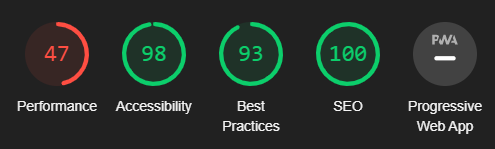
\includegraphics[scale=0.4]{img/first-result.png}
    \caption{First run of lighthouse testing}
    \label{fig10:res1}
\end{figure}

\begin{figure}
    \centering
    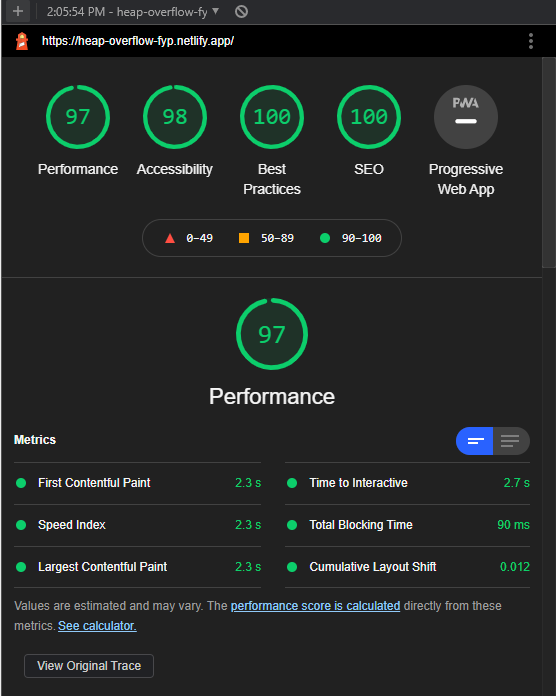
\includegraphics[scale=0.4]{img/result.png}
    \caption{lighthouse testing on finished project}
    \label{fig10.1:res2}
\end{figure}

\section{Limitations}
All applications have limitations, these limitations may surface during the development of the application or they have been foreseen before development. Some limitations that I had foreseen, is that there would not a sufficient amount of time to also tailor this application to be used by mobile phone users, which could cut-off an area of reach. While React does come with features that help rendering components on mobiles, when custom styling is added, those features or not helpful. Another limitation I encountered was the amount of work I could dedicate to this project as a single developer. Being a single developer, I had to develop all the functionality and design of the UI by myself while simultaneously working on other projects. If I was a member of a group, some of the features and functionalities could have been redistributed. Also, more features would have been implemented to make a more complete forum website. As at the moment the web application is limited to creating authenticated accounts, being able to post messages on the board, edit the user details and also the forum messages that were posted by that user. Another Limitation I identified is that it is not a Progressive Web Application. Progressive Web Applications are quickly becoming the standard, they have many functionalities like automatic HTTPS redirects, security improvements and they are able to be accessed even without an internet connection.
However coming into this project I had the objective of learning about the development of these complex web applications using a suite of different technologies, and being able to encounter these sort of limitations while developing this project provided some valuable insights to be taken on board for the future.


\chapter{Conclusion}
To conclude this paper, the objective was to create a forum web application using a variety of technologies to increase my skill set and use it as a learning experience to gain insight as to how complex modern day web applications are created. I managed to meet a lot of the objectives outlined
in the introduction and with the creation of this project I had some personal enlightenment. By developing this application I managed to gain some great insights into the development process of web applications. Some of these insights include structuring of the project being a very crucial part of the success. As I mentioned in the introduction, this project was not my initial idea. My initial project proposal was also another web application except it would have been created via Django and React working in tandem. When working with these two technologies, in a way they seemed incompatible. And after the development of this project, I believe it could be down to me not properly organising the project structure, that would have allowed me to work at it in a linear fashion. What I mean by this, is because of the way I had structured the Django React project I found myself hopping from the front-end to the back-end trying to figure out how everything connects together, without making much headway. Whereas in the case of this project "Heap-Overflow", I found it being an enjoyable experience working on it. By properly structuring the project, it eliminated the majority of confusion when having to link different components of the project together.

Changing my initial project and having to abandon what I had already developed was also a good experience to take away from this. Looking back in hindsight I believe it was the correct choice in my case. As I found myself stressing over the initial more and more each day, I came to the conclusion pretty late that it was best to abandon that endeavour. In abandoning it, I also gained more drive for developing this application, as I had a lot of work ahead of me, to catch up on.

By developing this application I was also exposed to an array of different technologies, even if I did not necessarily use them for development. As an example when researching the different stacks, primarily the MEAN stack and the MERN stack. While Angular is a full framework, it is actually more popular for creating small to medium range web applications. If I had realised the scope of the projects I was developing earlier, I would have considered the MEAN stack more seriously, but since I was so focused and determined to make a forum web application, I chose the MERN stack for the scalability and versatility reasons. 
The importance of planning was another big takeaway from this project, but also the ability to abandon something if it is not working, and it is hard to find motivation to do it. There was realisation that some documentation for technologies is easier to understand compared to others. But in general all the technologies I used during development all had great documentation.

Looking back, I would have also liked to work in a group, for a project like this. Some of the reasons would include having partners to bounce ideas around with. It would also give you a certain responsibility to uphold your end of the bargain when developing the application. As if that happens in a group you are responsible for slowing down the progress, whereas as a solo developer on a project all the responsibility is on yourself. This allows for laziness to creep in and then you end being behind schedule. Being in a group would also allow the delegation of different tasks and not to mention experience in working on a project as a team. Which would be very good preparation for entering a workplace.

While developing the project there were objectives that were not reached. They mainly pertained to the functionality of the website. One of these features include having the ability to comment on posts created by other users, and being able to uniquely identify the commenter using the web tokens. Although I did manage to achieve the objective of being able to identify specific users and allow them to interact with components of the page only they are privy to.

To conclude I managed to reach my main objective of learning about the development of web application. I took away many lessons like how to do research, how utilise different online resources and use it the application or having to drop a certain idea to start a new one to be able to progress. The experience and knowledge gained from developing this project will always be remembered.

